\graphicspath{{img/ch5}}
\section{Related Unmanned Missions}

The exploration of lunar pits and lava tubes has transitioned from observational curiosities to key objectives in planetary science and lunar exploration. These missions provide essential insights into the Moon’s volcanic history and potential access to subsurface voids.

\subsection{Past Missions}

\textbf{Apollo Program:}  
The Apollo program laid the foundation for modern lunar exploration by providing essential geological and subsurface data. Apollo 15 identified Hadley Rille, a collapsed lava tube, while Apollo 17’s Apollo Lunar Sounder Experiment (ALSE) utilized radar to detect subsurface voids and structural discontinuities, suggesting the presence of lava tubes and faults beneath the surface. ALSE's pioneering radar observations demonstrated the potential of subsurface mapping on the Moon and influenced the design of future missions, such as SELENE and Chang’e \cite{radar-observations-lava-tubes}.

\textbf{SELENE (Kaguya):}  
Japan's SELENE (Kaguya) mission, launched in 2007, provided groundbreaking evidence of intact lava tubes using the Lunar Radar Sounder (LRS). Double-echo radar patterns near the Marius Hills Hole (MHH) confirmed the existence of hollow subsurface structures, with void dimensions and roof thickness inferred from radar analysis. These findings offered unprecedented insights into lunar volcanic history and the stability of subsurface cavities. SELENE’s high-resolution imagery further complemented radar data, enabling detailed mapping of the lunar surface and its volcanic features \cite{cavities-selene-lavatubes, radar-observations-lava-tubes}.

\textbf{Chang’e Missions (China):}  
China’s Chang’e program advanced subsurface exploration through ground-penetrating radar (GPR) deployed on Chang’e-3 and Chang’e-4. These missions mapped regolith layers and detected subsurface voids, with Chang’e-4 providing unique data from the lunar far side. High-resolution radar from these missions revealed stratified geological layers and potential lava tube structures beneath the regolith, enhancing understanding of lunar geology and informing future mission planning \cite{radar-observations-lava-tubes, cavities-selene-lavatubes}.

\subsection{Active Missions}

\textbf{Lunar Reconnaissance Orbiter (LRO):}  
NASA’s LRO has played a pivotal role in mapping lunar pits and identifying their connections to subsurface features:
\begin{itemize}
    \item The \textbf{Narrow Angle Camera (NAC)} discovered over 300 pits, including the well-studied Mare Tranquillitatis pit \cite{thermal-lunar-pits}.
    \item The \textbf{Mini-RF radar} validated links between pits and lava tubes, emphasizing their significance for future exploration \cite{new-wagner}.
    \item The \textbf{Diviner Lunar Radiometer Experiment (DLRE)} revealed thermally stable environments within pits, highlighting their suitability for exploration and habitation \cite{thermal-lunar-pits}.
\end{itemize}

\begin{figure}[h!]
    \centering
    \begin{minipage}{0.48\textwidth}
        \centering
        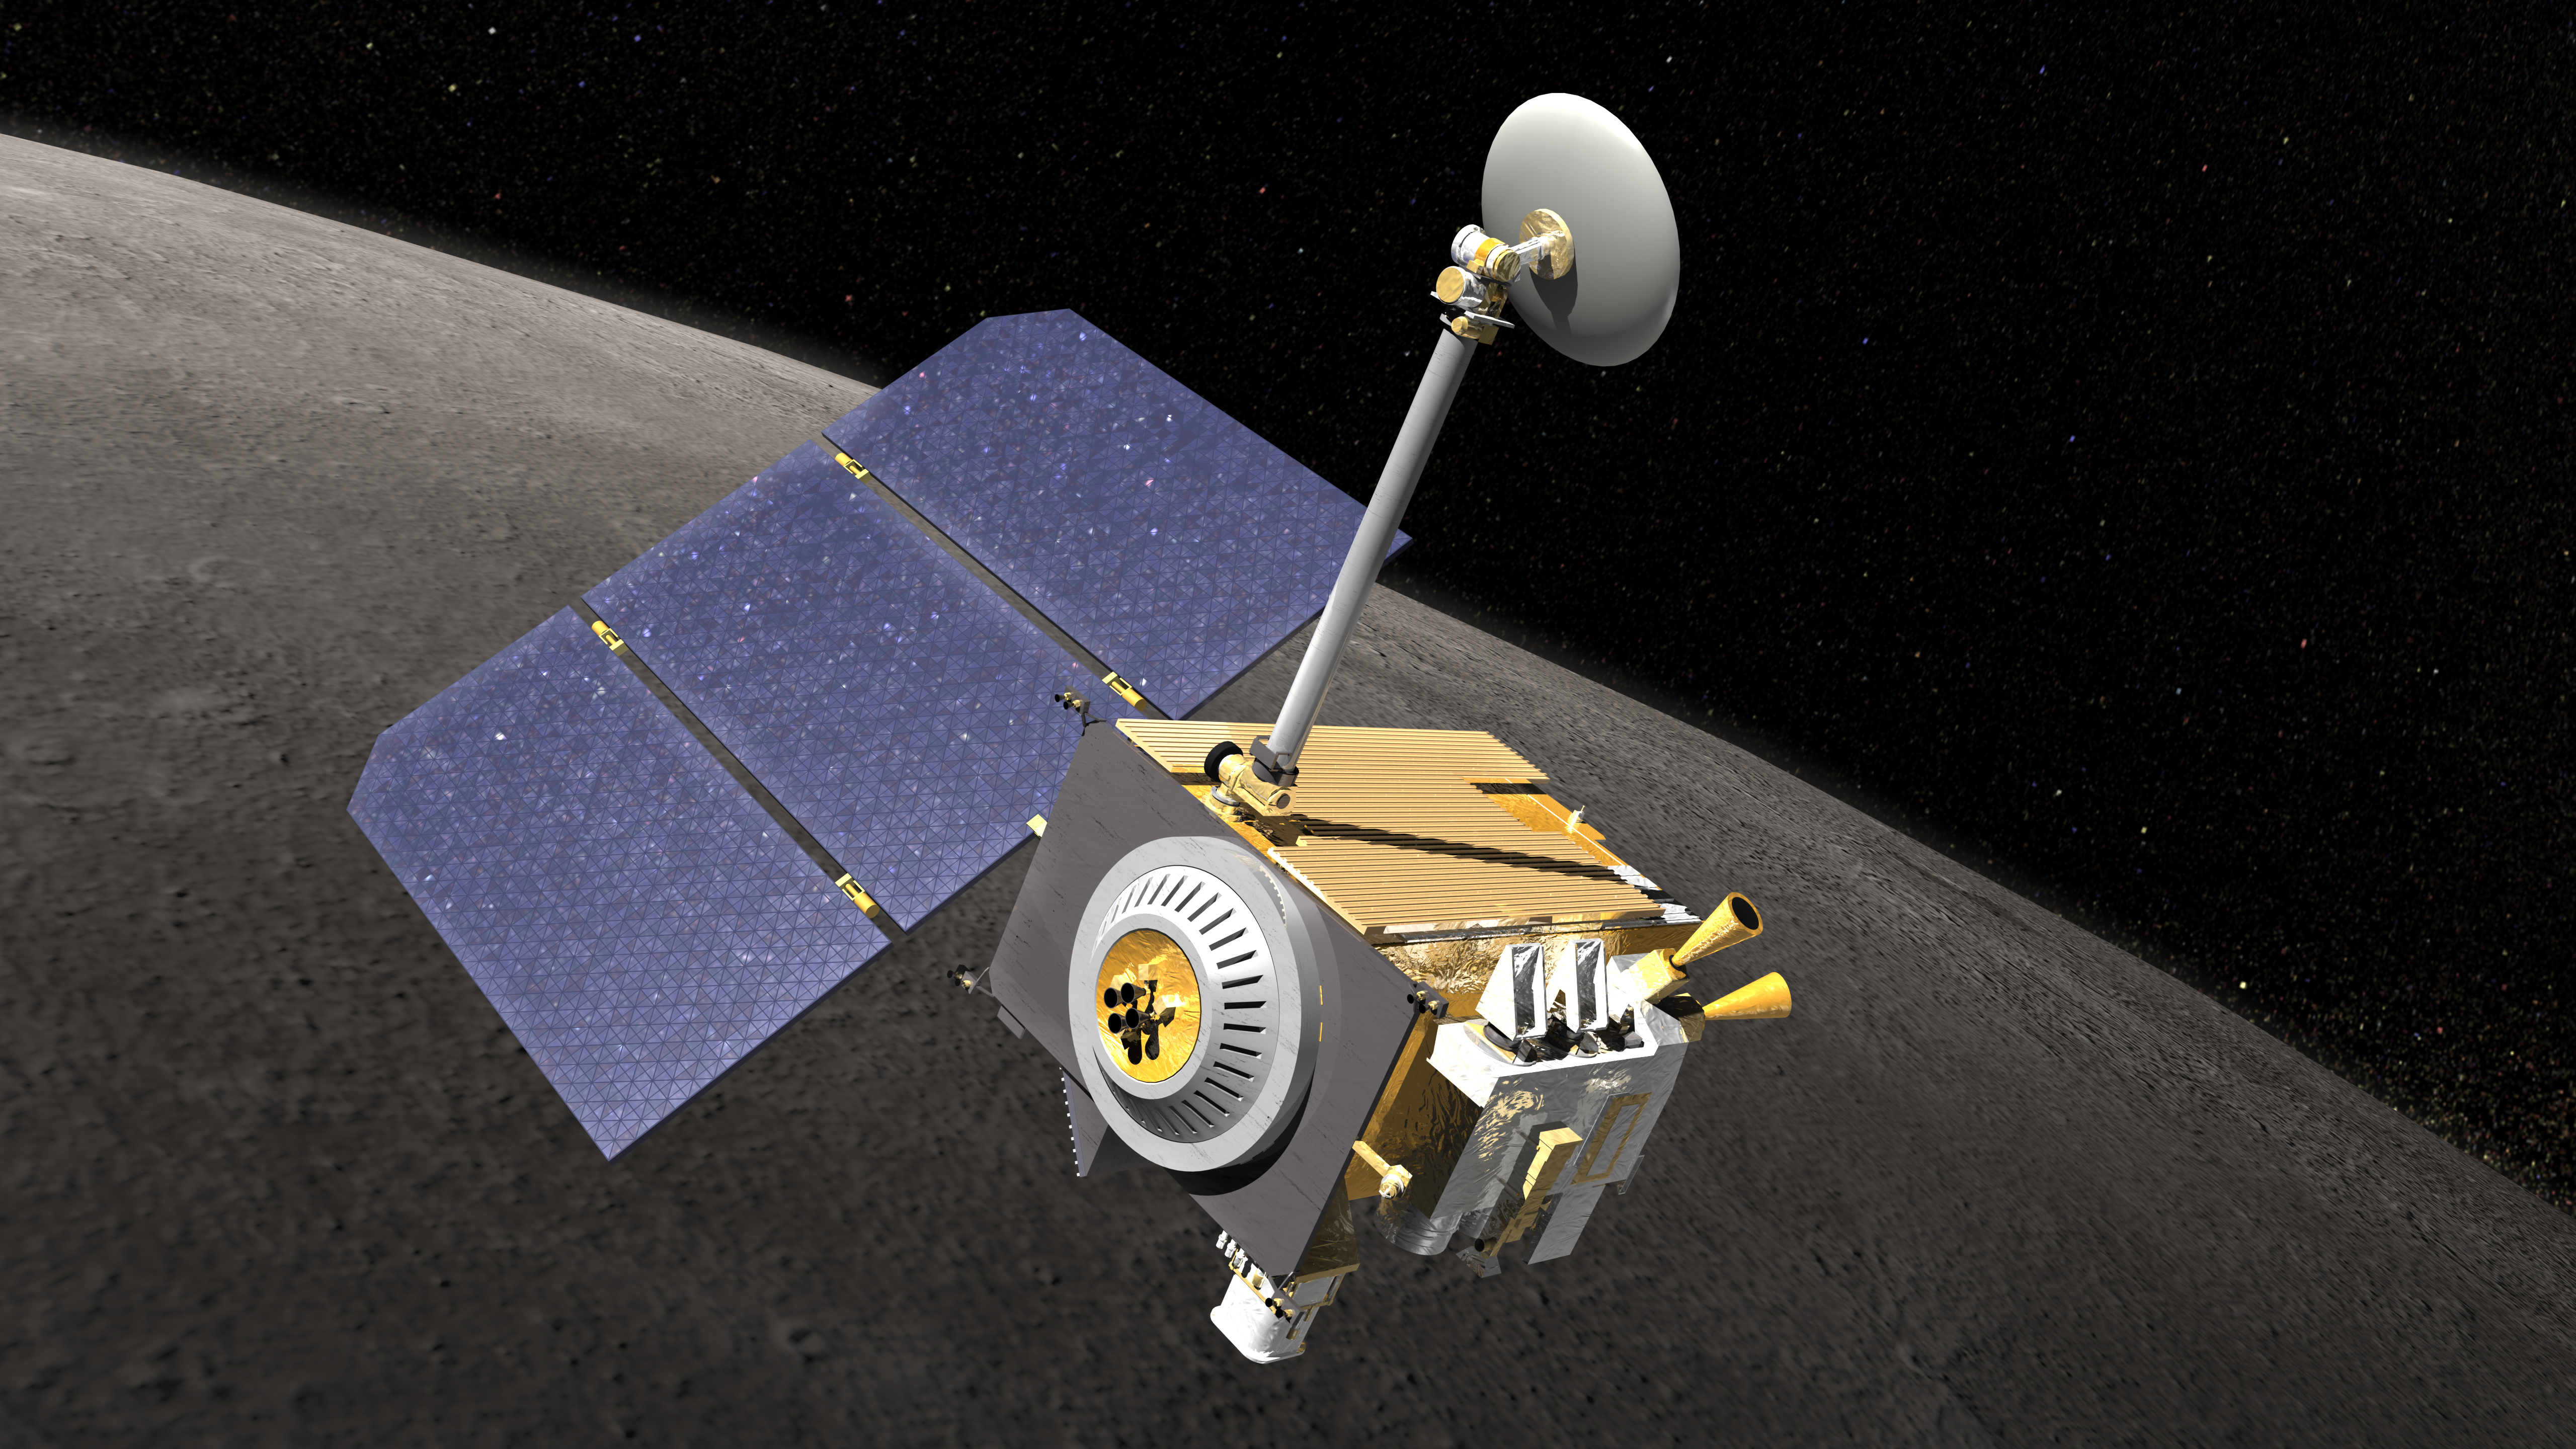
\includegraphics[width=\textwidth]{LROC-render.png}
        \caption{Artistic rendering of the Lunar Reconnaissance Orbiter (LRO) in lunar orbit, adapted from \cite{lro}}
        \label{fig:lro_render}
    \end{minipage}
    \hfill
    \begin{minipage}{0.48\textwidth}
        \centering
        \includegraphics[width=\textwidth]{LROC-schema.png}
        \caption{Schematic of LRO with labeled instruments, adapted from \cite{lro}.}
        \label{fig:lro_schema}
    \end{minipage}
\end{figure}

\textbf{GRAIL (NASA):}  
The Gravity Recovery and Interior Laboratory (GRAIL) mission utilized twin spacecraft, Ebb and Flow, to map the Moon's gravity field with unprecedented precision. Data from GRAIL revealed significant mass deficits beneath the Marius Hills region, strongly indicating the presence of extensive hollow structures, such as lava tubes, that could span up to 60 km in length \cite{grails-gradients-mariushills}.

\begin{figure}[H]
    \centering
    \includegraphics[width=0.52\linewidth]{grail.png}
    \caption{The GRAIL mission satellites used to measure the Moon’s gravity gradients \cite{GRAIL}.}
    \label{fig:grail-render}
\end{figure}

\subsection{Future Planned Missions}

\textbf{Daedalus Rover (ESA):}  
The European Space Agency’s (ESA) Daedalus (Descent And Exploration in Deep Autonomy of Lunar Underground Structures) rover is an advanced mission concept designed to explore the Marius Hills Pit. This skylight provides access to one of the Moon's most prominent lava tubes, making it an ideal candidate for investigating subsurface environments. The Daedalus mission seeks to autonomously map and analyze these environments \cite{esa-daedalus}.

The Daedalus rover is deployed via a tethered descent system to ensure precise placement and communication with the surface. Equipped with advanced 3D lidar and stereo cameras, the rover maps pit interiors and surrounding structures in high resolution, while also analyzing environmental conditions such as structural integrity, radiation, and thermal stability to assess habitability \cite{esa-daedalus}.

A unique feature of Daedalus is its swarm of kinetic energy-based jumping mechanism, which allows it to traverse rugged and uneven terrain. This capability enables it to navigate obstacles and confined spaces that are inaccessible to traditional rovers, making it ideal for exploring lava tubes and subsurface voids. Each jump is carefully controlled for stability and precision upon landing.

\begin{figure}[H]
    \centering
    \includegraphics[width=0.66\linewidth]{daedalus-schema.png}
    \caption{Conceptual diagram of the Daedalus rover’s exploration system, showcasing its tethered deployment and instrumentation \cite{esa-daedalus}.}
    \label{fig:daedalus-mission-schema}
\end{figure}

The jumping mechanism is illustrated below, showing its ability to adapt to challenging environments:

\begin{figure}[H]
    \centering
    \begin{minipage}[b]{0.2\textwidth}
        \centering
        \includegraphics[width=0.5\textwidth]{daedalus-jumper-1.png}
        \caption*{Static position}
    \end{minipage}
    \hspace{0.02\textwidth}
    \begin{minipage}[b]{0.2\textwidth}
        \centering
        \includegraphics[width=0.5\textwidth]{daedalus-jumper-2.png}
        \caption*{Preparing for a jump}
    \end{minipage}
    \hspace{0.02\textwidth}
    \begin{minipage}[b]{0.2\textwidth}
        \centering
        \includegraphics[width=0.5\textwidth]{daedalus-jumper-3.png}
        \caption*{Mid-air jump}
    \end{minipage}
    \caption{Stages of motion for the Daedalus jumping robot, highlighting its innovative locomotion system \cite{esa-daedalus}.}
    \label{fig:lunar_robot_movement}
\end{figure}

\textbf{Moon Diver Mission (NASA):}  
The Moon Diver mission, proposed by NASA, aims to deploy the Axel Extreme Terrain Rover into the Mare Tranquillitatis pit, a 125-meter-deep lunar mare pit with exposed basalt layers. This mission is designed to investigate the geological history and volcanic processes that shaped the Moon, with a particular focus on stratified lava flows visible within the pit walls \cite{kerber2023, nesnas2019}.

The Axel rover is a tethered robotic system uniquely engineered for extreme terrain exploration. Its innovative design includes:
\begin{itemize}
    \item \textbf{Tethered Descent System:} The rover is equipped with a 300-meter tether that provides both mechanical support and power, enabling controlled descent into steep-walled craters while maintaining uninterrupted communication with the lander \cite{kerber2016}.
    \item \textbf{Modular Mobility:} The rover’s dual-wheel configuration and detachable tether arm allow it to maneuver efficiently on uneven surfaces, ensuring adaptability in challenging lunar environments.
    \item \textbf{Scientific Payload:} The rover carries instruments such as the Multispectral Microimager (MMI) for high-resolution imaging of mineralogical features, an Alpha Particle X-ray Spectrometer (APXS) for elemental analysis, and FarCam and CloseCam cameras to document pit stratigraphy and generate 3D topographic models \cite{kerber2023}.
\end{itemize}


\begin{figure}[H]
    \centering
    \begin{minipage}[b]{0.49\textwidth}
        \centering
        \includegraphics[width=\textwidth]{moon-diver-pit-recon.png}
        \caption{3D reconstruction of a terrestrial pit using the Moon Diver prototype. This model demonstrates the rover’s capability to map pit stratigraphy with precision \cite{kerber2023}.}
        \label{fig:moon_diver_3d_recon}
    \end{minipage}
    \hfill
    \begin{minipage}[b]{0.49\textwidth}
        \centering
        \includegraphics[width=\textwidth]{moon-diver-schemoid.png}
        \caption{Schematic visualization of the Axel Rover’s tethered descent system, highlighting its mechanical and power supply features \cite{nesnas2019}.}
        \label{fig:moon_diver_schematic}
    \end{minipage}
\end{figure}

\subsection{Scientific Value of Lunar Pits and Lava Tubes}

Lunar pits and lava tubes provide exceptional opportunities for scientific research, offering unique insights into planetary geology, volcanism, and the Moon's evolutionary history.

\textbf{Preservation of Geological History:}  
The interiors of lava tubes and pits serve as natural archives of the Moon's volcanic activity. Their stable, unaltered environments protect geological features and stratigraphic layers, offering detailed records of past eruptions, lava flow dynamics, and crustal evolution \cite{thermal-lunar-pits, cavities-selene-lavatubes}.

\textbf{Understanding Lunar Volcanism:}  
The exposed layers within pits like the Mare Tranquillitatis provide access to stratified basalt flows, enabling detailed investigations of volcanic processes. These studies help to reconstruct the Moon’s thermal history and assess its geological diversity \cite{kerber2023, grails-gradients-mariushills}.

\textbf{Exploration of Subsurface Voids:}  
Subsurface cavities, identified through radar and gravity anomalies, allow researchers to study the structural integrity and formation mechanisms of large-scale lava tubes. These features highlight differences between terrestrial and lunar volcanism, particularly in terms of scale and stability, attributed to the Moon’s low gravity and lack of atmospheric erosion \cite{cavities-selene-lavatubes, grails-gradients-mariushills}.

\textbf{Astrobiological Potential:}  
The stable thermal environments and potential for volatile accumulation within pits make them analogous to habitable conditions on other celestial bodies. These studies inform astrobiological exploration and guide the search for life-supporting environments beyond Earth \cite{newer-thermal, sublunear-lava}.

\textbf{Comparative Planetology:}  
Lunar pits and lava tubes act as analogs for subsurface voids on other planets, such as Mars. The study of these features enhances our understanding of planetary processes and provides a framework for exploring similar structures on extraterrestrial surfaces \cite{cavities-selene-lavatubes, kerber2016}.
